\documentclass[12pt, letterpaper]{article}

\usepackage[utf8]{inputenc}
\usepackage[english]{babel}
\usepackage[T1]{fontenc}
\usepackage{graphicx}
\usepackage{tikz}
\usepackage{subfig}
\usepackage{wrapfig}
\usepackage{longtable}
\usepackage{amsmath}
\newcommand\tab[1][1cm]{\hspace*{#1}}
\renewcommand{\baselinestretch}{1.3}

\begin{document}

\begin{titlepage}

\begin{center}
	\large{EC336: Embedded Systems}\\
	\huge{\textbf{Interfacing Display Devices}}\\
	\large{Arvind S Kumar (15EC106), Pavan M (15EC137),\\ Samarth B (15EC143), Sripathi M (15EC149)}\\
	\large{22 August 2018}
\end{center}	

\begin{figure}[!h]
	\centering
	\includegraphics[scale=0.8]{/home/sripathi/GitHub_Repositories/NITK_Emblem.png}
	\label{fig:NITKEmblem}
\end{figure}	
\begin{center}
	
\huge{Submitted to:}\\
\begin{large}
Prof. Ramesh Kini M, Prof. Arulalan Rajan\\
Department of Electronics and Communication Engineering\\
NITK, Surathkal
\end{large}

\end{center}

\end{titlepage}

\section{Goal of the Lab}

The aim of this lab was to interface the chosen microcontroller with input devices such as the Hex keypad and the Keyboard. The microcontroller chosen by our group is TI's MSP430G2.

\section{Components Used}

For this lab the components used are :

\begin{itemize}
	\item MSP430 microcontroller
	\item LEDs
	\item 220 $\Omega$ resistors
	\item Hex Keypad
	\item Keyboard
\end{itemize}

\section{Board Details}

Some of the features of the MSP430 are - (Refer Figure \ref{fig:architecture} and Figure \ref{fig:board} for more information)

\begin{itemize}
	\item 16-bit RISC architecture
	\item Von-Neumann architecture
	\item Upto 16 MHz clock frequency
	\item Low power consumption and five power saving modes
	\item 16 general purpose registers
	\item 10-bit ADC
	\item Supports SPI, I2C, UART and USB interfaces
	\item Has 16 GPIO pins divided as two ports (8-bit each)
\end{itemize}
	
\begin{figure}[t]
	\centering
	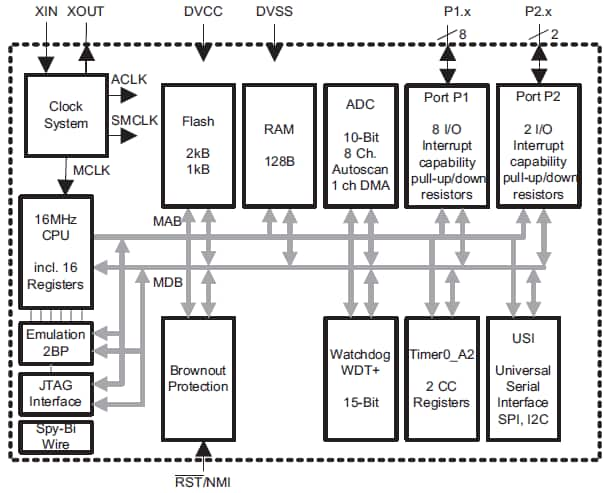
\includegraphics[scale=0.8]{/home/sripathi/GitHub_Repositories/Embedded-Systems/LatexFiles/msp430g2231-ep-ti.png}
	\caption{MSP430 Architecture}
	\label{fig:architecture}
\end{figure}

\begin{figure}[t]
	\centering
	\subfloat[fig:board][Board]{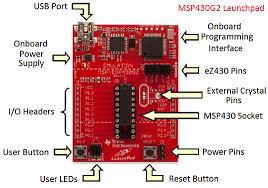
\includegraphics[scale=0.8]{/home/sripathi/GitHub_Repositories/Embedded-Systems/LatexFiles/board_msp430.jpeg}}
		\subfloat[fig:pindiagram][Pin Diagram]{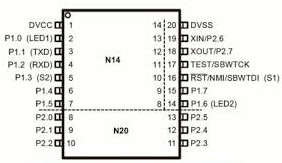
\includegraphics[scale=0.8]{/home/sripathi/GitHub_Repositories/Embedded-Systems/LatexFiles/pinout_msp430.jpeg}}
		\caption{Board details}
		\label{fig:board}
\end{figure}

\section{Interfacing Details}

Two input devices - the Hex Keypad and the Keyboard were interfaced. Both the devices were manufactured by Electro Systems, Bangalore and datasheets for the devices are available at the Embedded Lab. In order to observe the outputs of these devices, we also connected LEDs to the MSP430 and programmed a software decoder to translate key presses to a 4-bit binary value that were displayed using LEDs. 

\subsection{General layout}

The internal schematic for each of the devices discussed here will be elaborated in the respective sections. The general structure, however, is the same. Each of the keys act like push-buttons in the circuit. There are two controlling lines that help the user detect which key was pressed. The lines and the keys form a matrix. Each line controlling the rows are inputs and line controlling the columns are outputs from the peripheral. 

Initially, all the rows are enabled and the MSP waits for a key press. As soon as a key is pressed, the column is detected and to detect the row, the rows are enabled one by one and the column is monitored. The enabled row for which the column is also enabled, gives us the exact location of the key pressed.

VCC = 5V and GND are connected to the MSP 5V output (TP1) and GND respectively.  

\subsection{Hex Keypad}

The hex keypad is a 4x4 keypad with numbers from 0-9 and the hex digits A-F. Internally it is structured as 4x4 matrix. The rows are connected to Port 2 of the MSP and the columns are connected to Port 1 of the MSP. 4 LEDs are connected to Port 2 to display the decoded output. Port 2 is set to output and Port 1 to input. 

\subsection{Keyboard}

The keyboard is a 4x6 keyboard with numbers from 0-9, basic math operators - $ =, ., +, -, *, / $ and \% and some basic calculator operators M+, M-, MR, MC, AC, CE and CHK. Internally it is structured as 3x8 matrix. The rows are connected to Port 2 of the MSP and the columns are connected to Port 1 of the MSP. 4 LEDs are connected to Port 2 to display the decoded output. Port 2 is set to output and Port 1 to input. 

For ease of display and due to less number of pins available, the row controlling the calculator functions are disabled. (PC2)

The internal structure of the keyboard is as shown in Fig \ref{fig:keyboard}.

\begin{figure}[!h]
	\centering
	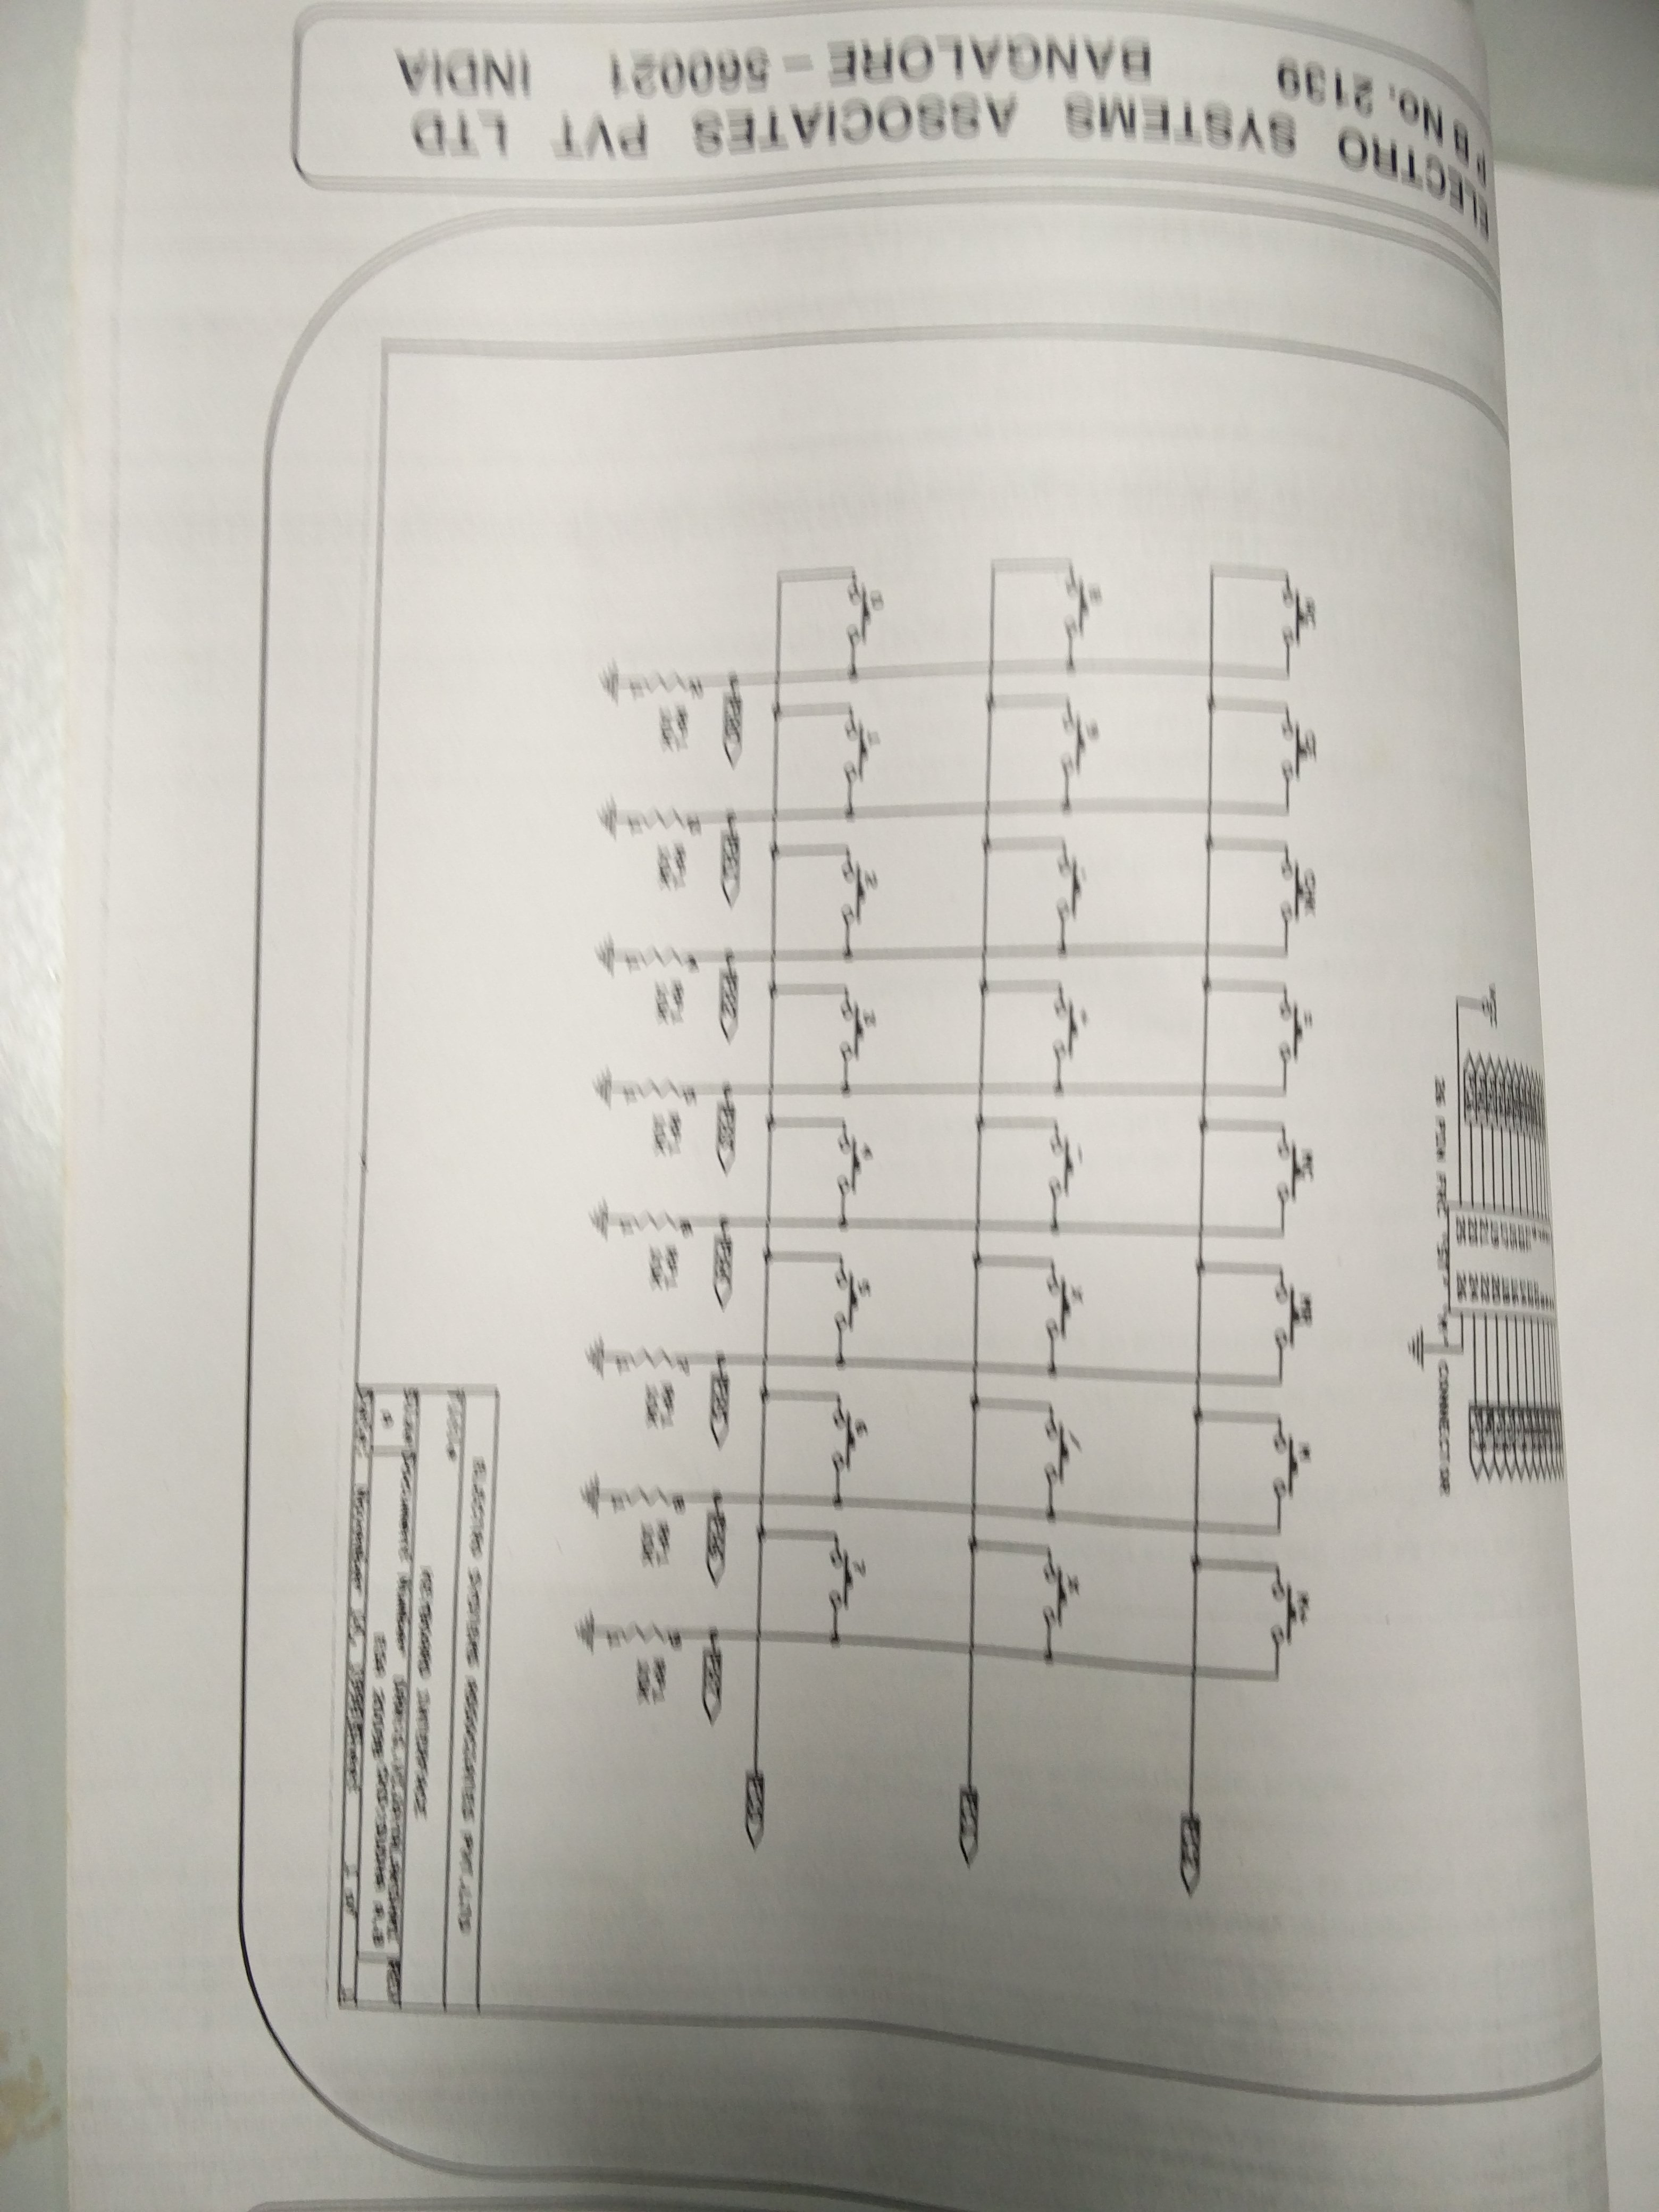
\includegraphics[scale=0.4, angle=90]{/home/sripathi/GitHub_Repositories/Embedded-Systems/LatexFiles/Interfacing_Input_Devices/Keyboard.jpeg}
	\caption{Keyboard}
	\label{fig:keyboard}
\end{figure}

\newpage

\section{Program}

Since the procedure for both the keypad and the keyboard are similar, the code here is presented for the more complex keyboard. 

%\begin{center}
\begin{longtable}{|p{8cm}||p{6cm}|}
%\caption{A sample long table.} \label{tab:long} \\

\hline 
\multicolumn{1}{|c|}{\textbf{Interfacing Keyboard using MSP430}} & \multicolumn{1}{c|}{\textbf{Pseudo code}}  \\ 

\hline 
\endfirsthead

\multicolumn{2}{c}%
{{\bfseries \tablename\ \thetable{} -- continued from previous page}} \\
\hline 
%\multicolumn{1}{|c|}{\textbf{First column}} & \multicolumn{1}{c|}{\textbf{Second column}} & \multicolumn{1}{c|}{\textbf{Third column}} \\ 
\hline 
\endhead

\hline \multicolumn{2}{|r|}{{Continued on next page}} \\ \hline
\endfoot

\hline \hline
\endlastfoot



\#include <msp430.h>  & \\             


int main(void)\{ & \\

   \hspace{0.1cm} WDTCTL $=$  WDTPW $|$ WDTHOLD;    & Stop watchdog timer \\ 

    
  \hspace{0.1cm}   P2DIR $=$ 0x3F;    & P2 0-3 used for rows (PCs - input, writing to it) \\ 
  \hspace{0.1cm}   P1DIR $=$ 0x00;       & P1 0-7 used for columns (PAs - output, reading from it) \\    
   \hspace{0.1cm} unsigned int output, i, column, row, tempP2OUT; & \\
    \hspace{0.1cm} unsigned int digits[2][8] $=$ \{\{0, 1, 2, 3, 4, 5, 6, 7\}, \{8, 9, 10, 11, 12, 13, 14, 15\}\}; & Array to store which row and column Corresponds to which Key on Keyboard\\
    
   \hspace{0.1cm} & \\
  \hspace{0.1cm}  for(;;) \{   &  Begin loop\\
  \hspace{0.1cm} & \\
     \hspace{0.3cm}   P2OUT $=$ 0x03; & Setting All Rows to high\\   
\hspace{0.1cm} & \\
     \hspace{0.3cm}   column $=$ P1IN; & Reading Column Input\\
     \hspace{0.1cm} & \\
      \hspace{0.3cm}  if(column $!=$ 0x00) \{ & Until Any of the Column is Triggered \\
\hspace{0.1cm} & \\
      \hspace{0.3cm}   switch(column) \{ & Finding out which column is triggered \\
        \hspace{0.5cm}     case 0x01: column $=$ 0; break; & \\ 
        \hspace{0.5cm}    case 0x02: column $=$ 1; break; & \\
        \hspace{0.5cm}   case 0x04: column $=$ 2; break;& \\
        \hspace{0.5cm}    case 0x08: column $=$ 3; break; & \\
        \hspace{0.5cm}    case 0x10: column $=$ 4; break & \\
        \hspace{0.5cm}    case 0x20: column $=$ 5; break; & \\
        \hspace{0.5cm}    case 0x40: column $=$ 6; break; &  \\
            \hspace{0.5cm}   case 0x80: column $=$ 7; break; & \\
            \hspace{0.5cm}     default: column $=$ 8; & Checking Condition for more than one column pressed\\
            \hspace{0.3cm} \} & \\
            
            \hspace{0.3cm}    if(column $!=$ 8) \{  & if more than one column is not pressed \\
            \hspace{0.5cm}     P2OUT $=$ 0x00; & Setting All Rows \\
            \hspace{0.5cm}    for(i $=$ 0; i $<=$ 1; i++) \{ & Setting rows ON one by one to find out which row is pressed\\
            \hspace{0.7cm}    P2OUT $=$ 0x02 $>>$ i; & \\
            \hspace{0.7cm}    if(P1IN $!=$ 0x00) & \\
            \hspace{0.9cm}    row $=$ i;     &  \\
            \hspace{0.7cm}    \} & \\
            \hspace{0.5cm}    \} & \\
            \hspace{0.3cm}    tempP2OUT $=$ (digits[row][column] $<<$ 2) \& 0x3C; & \\
            \hspace{0.3cm}    P2OUT $=$ 0x20 $^\wedge$ tempP2OUT; &  Setting Out Accordingly to turn on Externally Connected LEDs\\
            \hspace{0.3cm}    \} & \\

            \hspace{0.1cm}    \} & \\
            \hspace{0.1cm}     return 0; & \\
            \} & \\

\end{longtable}
%\end{center}

\section{Knowledge gained}

\begin{enumerate}
	\item Learnt how keyboard and keypad is designed and controlled.
	
	\item Understood the importance of datasheet and that it must be followed to the dot. For example, while interfacing the keyboard, the datasheet showed that the schematic was for a 3x8 key matrix whereas what we had on the board was a 4x6 matrix. We wasted a lot of time since we didn't believe the datasheet.
	
	\item Learnt the importance and need for debouncing. Hardware debouncing can be implemented using latches embedded in the keyboard or software debouncing using polling and delays. 
	
\end{enumerate}

\end{document}
